We consider the same systematics sources compared to the 
SM Higgs analysis~\cite{HWWHCP2012} for backgrounds. 
For signal shapes of exotic resonances we apply additional 
shape systematics to account for the missing high order effects. 
As discussed in Section~\ref{sec:datasel} we reweighted the $m_T-m_{\ell\ell}$ templates 
derived in JHUGen-Pythia to match to the predictions by Powheg-pythia samples in 
the SM Higgs hypothesis. 
The relative differences observed in the SM Higgs case are then 
applied to the other non-SM Higgs resonances. 
For the non-SM Higgs hypotheses we consider the JHUGen-Pythia 
predictions without reweighting as the $+1\sigma$ deviations from the central shapes. 
The correspoinding $-1\sigma$ variation is taken as the mirrored difference between 
the central and the $+1\sigma$ difference. 
Figure~\ref{fig:xwwshapevar} shows the central and the $\pm1\sigma$ variations 
of the $gg\to \text{Graviton}\to WW$ process. 

%%%%%%%%%%%%%%%%%%%%%%%%%%%%%%%%%%%%%%%%%%%%%
\begin{figure}[!hbtp]
\centering
\subfigure[]{
\centering
\label{subfig:xwwshapevar}
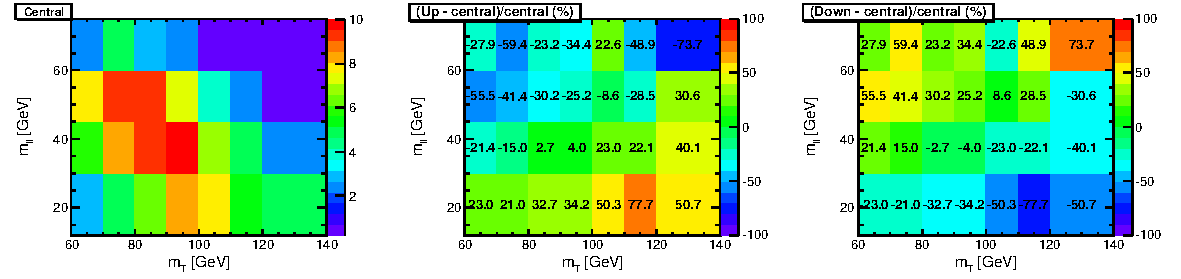
\includegraphics[width=1.15\textwidth]{figures/xww_ggHshapevar.pdf}
}
\caption{The shape variations for the $gg\to \text{Graviton}\to WW$. 
}
\label{fig:xwwshapevar}
\end{figure}
%%%%%%%%%%%%%%%%%%%%%%%%%%%%%%%%%%%%%%%%%%%%%
